% Test Plan: Proposed Security Enhancements for DCE DFS (OSF-RFC 90.0)
% Copyright (C) 1996 Transarc Corporation - All rights reserved

\documentstyle[titlepage,psfig]{article}

\begin{document}

\title{Test Plan for OSF-RFC 90.0\\
Security Enhancements for DCE DFS}

\author{Transarc Corporation\\
\\
\copyright 1996 Transarc Corporation}
\date{April 1996}

\maketitle

%
% ------------------------------------------------------------------------
%

\section{INTRODUCTION}

This document describes a plan for testing the implementation
of OSF-RFC~90.0\footnote{C. Everhart. {\em Proposed Security Enhancements
For DCE DFS.} OSF-RFC~90.0.  January 1996.}, security enhancements for DFS.
The test suite presented is intended to supplement existing
tests, in that it focuses only on exercising code paths that implement
the specified security enhancements.

Section~\ref{sec:config} presents an overview of the DCE/DFS configuration
utilized by all tests in the suite.
Section~\ref{sec:suite} describes the test suite in detail.

It is assumed that the reader is familiar with the details of OSF-RFC~90.0.

%
% ------------------------------------------------------------------------
%

\section{TEST CONFIGURATION}
\label{sec:config}

Figure~\ref{fig:config} depicts the DCE/DFS configuration required by
the test suite.  Two cells are needed,
one containing at least two DFS server machines ($A$ and $B$),
and the other containing at least one DFS server machine ($C$).
Tests are executed on machine $A$, which is considered to reside
in the local cell.

\begin{figure} [b]
\begin{center}
\leavevmode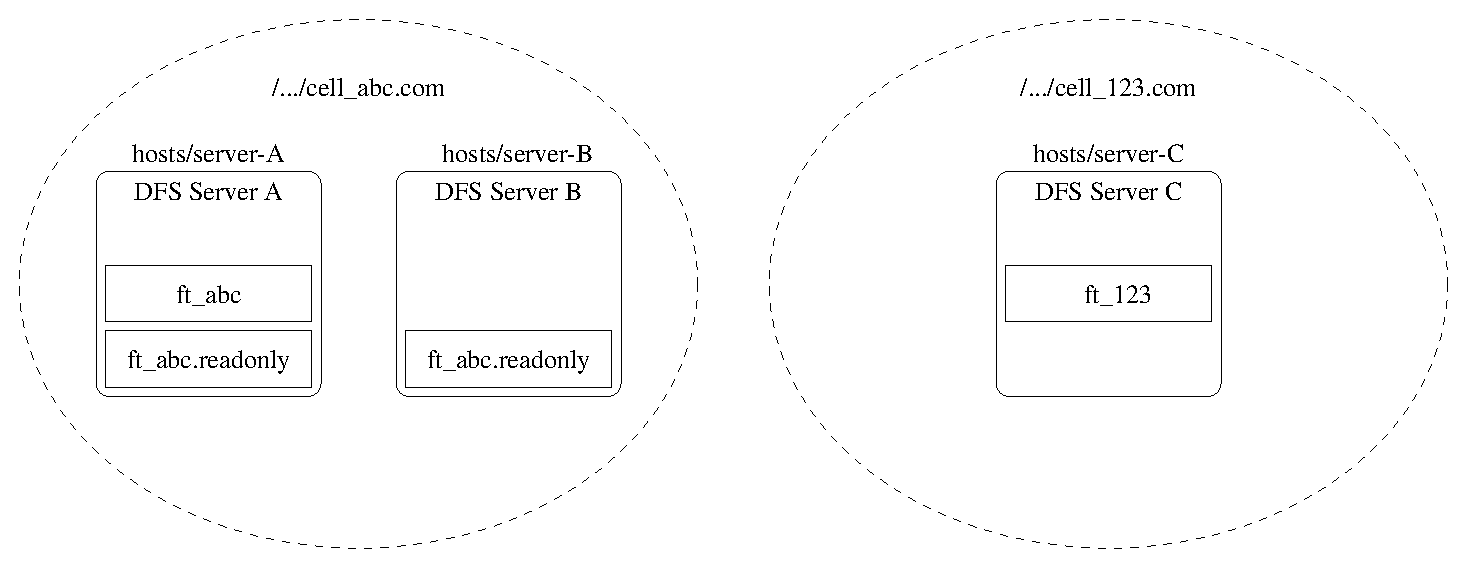
\psfig{file=config.ps,width=0.89\textwidth}
\caption{Enhanced DFS Security Test Configuration}
\label{fig:config}
\end{center}
\end{figure}

Tests operate on filesets
{\tt ft\_abc}, a schedule-replicated fileset in the local cell,
and {\tt ft\_123}, a non-replicated fileset in the foreign cell.
Throughout this text, file names have a suffix which indicates the
fileset to which the file belongs.  For example, if {\tt fred} is
a file in {\tt ft\_abc}, then the read-write copy of {\tt fred} is
referred to as {\tt fred.ft\_abc} and a read-only copy of {\tt fred} is
referred to as {\tt fred.ft\_abc.readonly}.  Similarly, server names
may have a suffix which indicates the machine on which they execute.
For example, a {\tt repserver} executing on machine $A$ may be
referred to as {\tt repserver-A}.


%
% ------------------------------------------------------------------------
%

\section{TEST SUITE}
\label{sec:suite}

This section describes a collection of tests designed to exercise
the code paths that implement all security enhancements described
in OSF-RFC~90.0.  An attempt has been made to categorize the various
security enhancements, and tests are grouped accordingly.

\subsection{User Interface Extensions}

\begin{sloppypar}
Administrators control DFS authentication via several new
commands and command-options.  Thus tests are needed to verify that
valid command arguments are accepted, and that invalid arguments are
rejected.  Note that these tests do not check that specified
authentication parameters are actually obeyed; this is the subject of
later tests.
\end{sloppypar}

\subsubsection{Startup-options test}

The {\tt dfsd} and {\tt fxd} commands both accept options that
specify authentication-level
bounds for CM-FX communications\footnote{Authentication-level bounds
can always be specified for both intra-cell and inter-cell communications.}.

This test verifies that only valid authentication-level
bounds can be specified, in any of the numeric, short or long forms;
for example `5', `{\tt pkt\_integ}'
or `{\tt rpc\_c\_protect\_level\_pkt\_integ}'.

To accomplish this task, the test executes,
as a non-root user, the {\tt dfsd} and {\tt fxd}
commands with various authentication arguments.
In determining if the commands behave properly,
the test is able to distinguish between failures due to
invalid arguments and failures due to having insufficient privilege to
execute the start-up system calls.

\subsubsection{Set-protection test}

\begin{sloppypar}
The {\tt cm} command implements a {\tt setprotectlevels} and
a {\tt getprotectlevels} subcommand for specifying and querying CM
authentication-level bounds for CM-FX communications.
Similarly, the {\tt fts} command implements a {\tt setprotectlevels}
subcommand for specifying per-fileset advisory authentication bounds.
\end{sloppypar}

This test verifies that only valid authentication-level bounds can
be specified, again in any of the numeric, short or long forms.

The test checks the output of either a {\tt cm getprotectlevels} or
a {\tt fts lsfldb} command, as appropriate, to determine if a
valid {\tt setprotectlevels} has actually set the authentication-level
bounds as specified.



\subsection{User-space Server RPC Authentication}

\begin{sloppypar}
The DFS security enhancements should ensure that DFS no longer employs
unauthenticated DCE RPCs for communication with user-space server processes.
Thus tests are needed to verify that previously unauthenticated RPCs are
now performed at the recommended authentication level
of {\tt rpc\_c\_protect\_level\_pkt\_integ} (or greater).
\end{sloppypar}

\subsubsection{Repserver-authentication test}

This test verifies that the {\tt fts}, cache-manager and {\tt repserver}
clients now all make authenticated {\tt repserver} RPCs.

Table~\ref{tbl:repauthn} depicts a sequence of commands that results in
a {\tt repserver} RPC by each each of the clients named above.
After executing
these commands, the test checks the {\tt repservers'} trace logs to determine
if the RPCs were indeed authenticated at the expected level.

\begin{table}[h]
\begin{tabular}{|p{1.5in}|p{3.0in}|}
\hline
\multicolumn{1}{|c|}{Action} & \multicolumn{1}{c|}{Result} \\
%
\hline
{\raggedright fts setrep ft\_abc [{\em arg}]} &
{\raggedright fts makes REP\_AllCheckReplicationConfig RPC
to repserver-A;\\
repserver-A makes REP\_CheckReplicationConfig RPC
to repserver-B} \\
%
\hline
{\raggedright cat fred.ft\_abc.readonly;\\touch fred.ft\_abc} & \\
%
\hline
{\raggedright sleep {\em maxage-of-ft\_abc}} & \\
%
\hline
{\raggedright cat fred.ft\_abc.readonly} &
{\raggedright CM makes REP\_GetVolChangedFiles RPC
to repserver-A} \\
%
\hline
\end{tabular}
\caption{Repserver-authentication test}
\label{tbl:repauthn}
\end{table}


% break page for formatting

\newpage


\subsubsection{Flserver-authentication test}

This test verifies that the cache-manager client now makes authenticated
{\tt flserver} RPCs.

Table~\ref{tbl:flauthn} depicts a sequence of commands that results in
a {\tt flserver} RPC by the cache-manager.
After executing these commands, the test checks the CM trace log to
determine if the RPC was authenticated at the expected level.

%\footnote{{\tt Flservers} do not log client authentication
%information, as do {\tt repservers}; hence the need to check
%the CM trace log.}.

\begin{table}[h]
\begin{tabular}{|p{1.5in}|p{3.0in}|}
\hline
\multicolumn{1}{|c|}{Action} & \multicolumn{1}{c|}{Result} \\
%
\hline
{\raggedright cm checkf} & \\
%
\hline
{\raggedright cat fred.ft\_abc.readonly} &
{\raggedright CM makes VL\_GetEntryByName RPC} \\
%
\hline
\end{tabular}
\caption{Flserver-authentication test}
\label{tbl:flauthn}
\end{table}


\subsection{Token-revoke RPC Authentication}

The DFS security enhancements should ensure that the DFS file-exporter
no longer employs unauthenticated DCE RPCs for token-revocation, except when
dealing with older clients.
Thus a test is needed to verify that token revokes to updated clients
are now performed at the recommended authentication level
of {\tt rpc\_c\_protect\_level\_pkt\_integ} (or greater).

\subsubsection{Token-revoke authentication test}

This test verifies that the {\tt fts}, {\tt dfsexport}, cache-manager
and {\tt repserver} clients now supply a principal name
in {\tt AFS\_SetContext} calls so that the file-exporter can authenticate
token-revoke binding handles.

Table~\ref{tbl:revokeauthn} depicts an action for each of the token
clients named above that
causes a file-exporter to create a `{\tt fshs\_host}' object for
the client, and subsequently authenticate its token-revoke binding handle.
After executing each of these commands, the test checks the
file-exporter's trace log to determine if the binding handles
were indeed authenticated at the expected level.

\begin{table}[h]
\begin{tabular}{|p{1.5in}|p{3.0in}|}
\hline
\multicolumn{1}{|c|}{Token Client} & \multicolumn{1}{c|}{Action} \\
%
\hline
{\raggedright fts} & {\raggedright fts clone ft\_abc} \\
%
\hline
{\raggedright dfsexport} &
{\raggedright dfsexport -aggr {\em server-A-aggr} -detach;\\
dfsexport -aggr {\em server-A-aggr}}  \\
%
\hline
{\raggedright repserver} &
{\raggedright bos restart /.:/hosts/server-A -proc repserver} \\
%
\hline
{\raggedright CM} &
{\raggedright (To be determined; will likely have to force new
principal binding authn and check CM trace log)} \\
%
\hline
\end{tabular}
\caption{Token-revoke authentication test}
\label{tbl:revokeauthn}
\end{table}


\subsection{CM-FX Authentication Negotiation}

As mentioned previously, administrators can control DFS communications
protection by specifying authentication-level bounds for
cache-managers and file-exporters; per-fileset advisory
authentication-bounds can be specified as well.

DFS security enhancements should ensure that CM-FX communication
occurs at a protection level that falls within the intersection
of a cache-manager's and file-exporter's bounds.  Note that the CM does
not specify an upper-bound on authentication-level, but rather an initial
bound that is the preferred starting point; effectively the CM can be viewed
as having an upper-bound of the maximum protection
level (rpc\_c\_protect\_level\_pkt\_privacy).

The following tests verify that CM-FX authentication-level is negotiated
as expected.  All tests are executed for both intra-cell and inter-cell
access, by principals that fall into the four logical
credential-categories: unauthenticated non-local-root, unauthenticated
local-root, DCE-authenticated non-local-root and DCE-authenticated
local-root.  DFS ACLs are presumed to be set so as to allow
unauthenticated access to files in the test
filesets ({\tt ft\_abc}, {\tt ft\_123}).
Accessing files unauthenticated allows the test to check that
protected communication is used for unauthenticated access, via the
method described in OSF-RFC~90.0.

\subsubsection{Non-intersecting protection-bounds test}

This test assigns a CM-FX pair various non-intersecting authentication-bounds
and checks that files can not be accessed (EACCESS) from the file-exporter.

Note that there is no command to dynamically alter a file-exporter's
authentication bounds.  Fortunately, these bounds can be patched
in the kernel via {\tt adb}.

\subsubsection{Intersecting protection-bounds test}

This test assigns a CM-FX pair various intersecting authentication-bounds
and checks that files can be accessed from the file-exporter.

The test examines CM and/or FX trace logs to determine that RPCs
occurred at the expected authentication level.

\subsubsection{Fileset protection-bounds test}

This test assigns a CM-FX pair fixed, intersecting authentication-bounds.
Various per-fileset authentication bounds are assigned to a fileset residing
on the FX, and files are accessed from it to check the influence
of these advisory bounds.

The test examines CM and/or FX trace logs to determine that RPCs
occurred at the expected authentication level.



%
% ------------------------------------------------------------------------
%

\end{document}
